\section{Task Definition}
\label{sec:task}
%The temporally ordered user interactions lead to the streaming nature of session data. Therefore it's natural and realistic to formulate the news recommendation task as a session-based recommendation task to predict next-item. 

Assume that an anonymous user $u$ produces a sequence of click events $S_u$, 
which can be represented as \[S_u: (n_1^u,c_1^u,t_1^u)\rightarrow(n_2^u,c_2^u,t_2^u)\rightarrow...\rightarrow(n_i^u,c_i^u,t_i^u),\] 
where $n_i^u$ is the id of the $i$-th news articles that user $u$ clicks, 
$c_i^u$ denotes the content representation vectors of the corresponding articles, and $t_i^u$ denotes the temporal information of the click event. The articles that appear in user $u$'s impression list are denoted as set $Imp_u$. An impression list is the articles in the vincinity of the articles
being clicked, which may have left an impression on the user.

For brevity, we ignore the $u$ superscript when discussing the information
for any user. The temporal information $t_i$ is a triple. 
The first part is the \textit{click time}: $tc_i$ of the $i^{th}$ click, and $tc_1$ means the start of session $S$, later we use click time $tc$ without subscript to stand for the start time of the session. The next is the 
\textit{publish time} $tp_i$, reflecting how fresh the $i^{th}$ article is compared with the current time. Last $ta_i$ is the \textit{active intervals} the user stays in $i$-th article. When $ta_i$ is not available, it can be infered from the difference of $tc_i$ and $tc_{i-1}$.

In the training phase, the recommendation system aims to model the 
user feedback sequence. While in test phase, 
given a target user $u$ with interaction sequence $S_u$ as input, 
our next-item recommendation task is 
to predict $n_{i+1}^u$ that the target user $u$ is most likely to click next. 
Noted that each user $u$ only appears once, 
which means training set and test set don't share the same users. 
The whole procedure is depicted in \figref{fig:task}.

\begin{figure}[th]
    \centering
    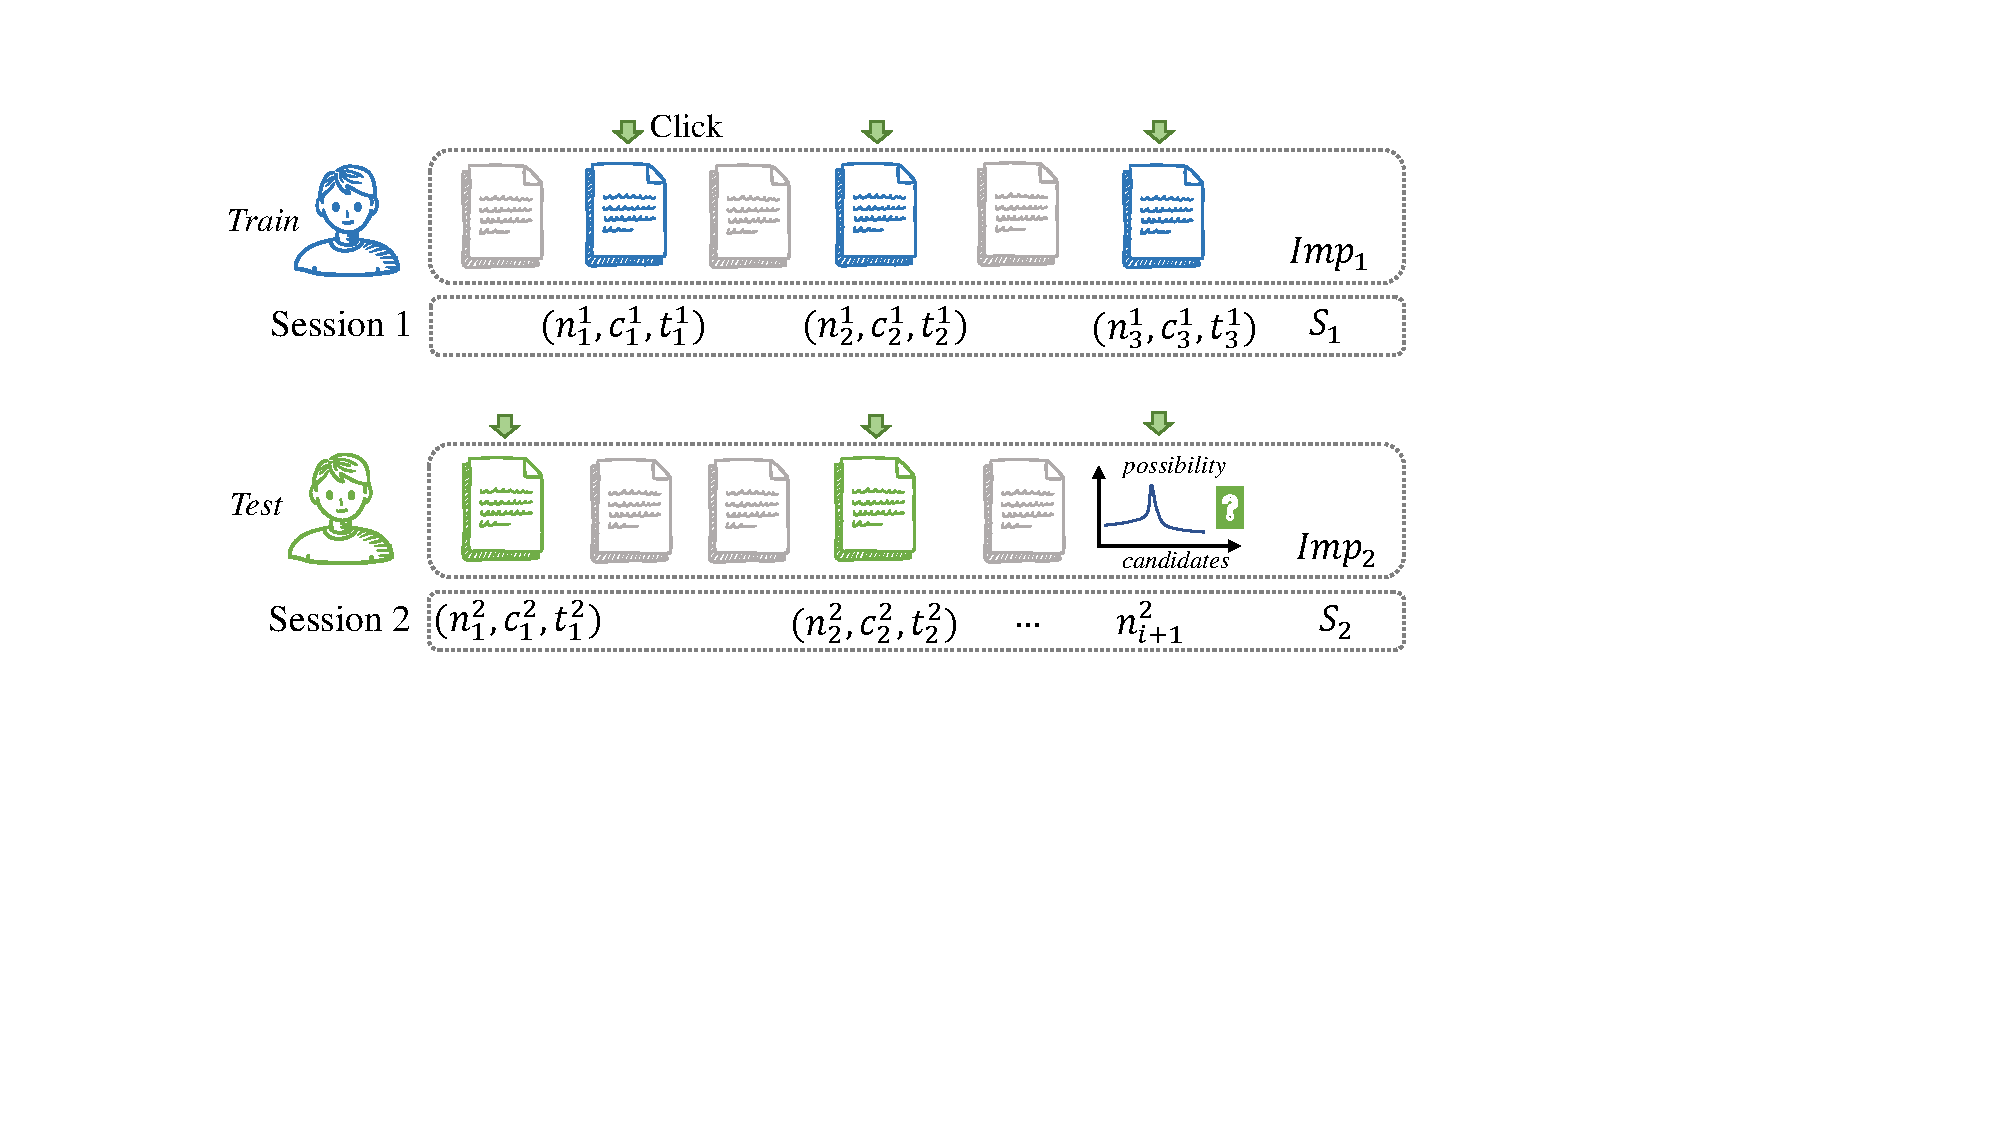
\includegraphics[width=\columnwidth]{fig/task.pdf}
    \caption{Session-based news recommendation procedure.}
    \label{fig:task}
\end{figure}
